%  This LaTeX template is based on T.J. Hitchman's work which is itself based on Dana Ernst's template.  
% 
% --------------------------------------------------------------
% Skip this stuff, and head down to where it says "Start here"
% --------------------------------------------------------------
 
\documentclass[12pt]{article}
 
\newcommand\tab[1][1cm]{\hspace*{#1}}
\usepackage[margin=1in]{geometry} 
\usepackage{amsmath,amsthm,amssymb}
\usepackage{graphicx}
\usepackage{subcaption}
\usepackage{siunitx}
\usepackage{pgfplots}
\pgfplotsset{compat=1.16}
\newenvironment{statement}[2][Statement]{\begin{trivlist}
\item[\hskip \labelsep {\bfseries #1}\hskip \labelsep {\bfseries #2.}]}{\end{trivlist}}

\usepackage[
sorting = none,
backend=bibtex,
natbib=true,
]{biblatex}
\addbibresource{bib.bib}
\begin{document}
 
% --------------------------------------------------------------
%
%                         Start here
%
% --------------------------------------------------------------
 
\title{HW2} 
\author{William Strickland}
\maketitle

\section{Newman 6.11}
\renewcommand\thesubsection{a}
\subsection{}
Starting with Eqn. (6.81) from Newman, we can say:

\begin{equation}
x^* = x_i + \epsilon_i
x^* = x_{i+1} + \frac{\epsilon_{i+1}}{(1+w)f'(x)-w}
\end{equation}{}
Using:

\begin{equation}
    x_{i+1} = (1+w)f(x_i)-wx_i
\end{equation}{}
and
\begin{equation}
    x^* = (1+w)f(x^*)-wx^*
\end{equation}
We can solve for $\epsilon_{i+1}$
\begin{equation}
    x_i+\epsilon_i = x_{i+1}+\epsilon_{i+1}
\end{equation}{}
\begin{equation}
    x_i+\frac{\epsilon_{i+1}}{(1+w)f'(x_i)-w} = x_{i+1}+\epsilon_{i+1}
\end{equation}{}
\begin{equation}
        \frac{\epsilon_{i+1}}{(1+w)f'(x_i)-w} - \epsilon_{i+1}= x_{i+1} - x_i
\end{equation}{}

\begin{equation}
        \epsilon_{i+1} \left( \frac{1}{(1+w)f'(x_i)-w} - 1 \right)= x_{i+1} - x_i
\end{equation}{} 
Now we see that
\begin{equation}
        \epsilon^* = \epsilon_{i+1} =  \frac{x_{i+1} - x_i}{(1/((1+w)f'(x_i)-w) - 1}
\end{equation}{} 

\renewcommand\thesubsection{b}
\subsection{}
We would like to find values of $x$ which solve the equation 

\begin{equation}
    x = 1 - e^{-cx}
\end{equation}{}
for $c = 2$.
To do this, we use the method of relaxation. We want to also know how many iterations it takes to solve this. One can see in Figure~\ref{fig:6.11b} that using the relaxation method took 14 iterations to converge to the right solution. The relaxation method was used with a starting value $x_0 = 1$.
\renewcommand\thesubsection{c}
\subsection{}
Now we would like to compare our results using the overrelaxation method. This method uses a parameter $\omega$, which helps us converge to the correct value of x faster, as seen in Figure ~\ref{fig:6.11c}. This method was computed for a starting value $x_0$ = 1, and $\omega$ = 0.5.

\begin{figure}
    \centering
    \begin{subfigure}[b]{0.4\textwidth}
        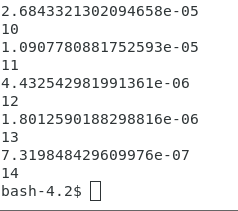
\includegraphics[width=\textwidth]{HW2_611_b.png}
        \caption{Relaxation method, the first value is the difference of the old x and the new x, while the second value is the iteration number}
        \label{fig:6.11b}
    \end{subfigure}
    ~ 
    \begin{subfigure}[b]{0.4\textwidth}
        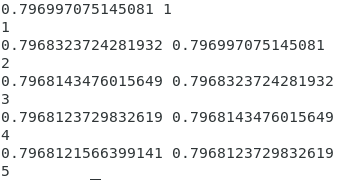
\includegraphics[width=\textwidth]{HW2_611_c.png}
        \caption{Using the overrelaxation method, the number of iterations decrased from 14 to 5. The first two values are the the old and new xs, while the second value is the iteration number}
        \label{fig:6.11c}
    \end{subfigure}
    \end{figure}

\renewcommand\thesubsection{d}
\subsection{}
Using $\omega < 1$ will help in cases where we overestimate the solution x. If we use $\omega > 1$, we will bounce around the solution for a long time before getting to the true solution. However, using $\omega<1$ will take an overestimate, and bring us closer to the original value.


\section{Newman 6.13}
\renewcommand\thesubsection{a}
\subsection{}

Planck's radiation law is given by:
\begin{equation}
     I(\lambda,T) =\frac{2 hc^2}{\lambda^5}\frac{1}{ e^{\frac{hc}{\lambda k_BT}}-1}
\end{equation}{}
Differentiating this function with respect to the wavelength, we can find the wavelength that maximizes the intensity of emitted radiation.
\begin{equation}
    \frac{dI}{d\lambda} = 5e^{-\frac{hc}{\lambda kT}}+\frac{hc}{\lambda k_BT} - 5 = 0
\end{equation}{}
Substituting
\begin{equation*}
    x = \frac{hc}{\lambda k_BT}
\end{equation*}
We can solve equation 11 for the wavelength.
\begin{equation}
    \lambda = \frac{hc}{xk_BT} = \frac{b}{T}
\end{equation}{}


\renewcommand\thesubsection{b}
\subsection{}
Using the binary search method, we can solve this equation for lambda. My binary search started in the interval [x=1,x=7], and I got a value for
\begin{equation}
    b = 0.002900
\end{equation}{}

\renewcommand\thesubsection{c}
\subsection{}
Plugging this value back into equation 12, and solving for T with a wavelength of 502 nm, we get
\begin{equation}
    T = 5776 K
\end{equation}{}
This value agrees very well with the expected value for the temperature of the sun, which is 5778 K\footnote{https://web.archive.org/web/20100715200549/http://nssdc.gsfc.nasa.g forked from jltinker/CompPhys2019
ov/planetary/factsheet/sunfact.html}

\newpage
\section{Fitting $\chi^2$ of the Schechter function}
This question involved work with the Schechter function, which tells you the inverse of the density of some galaxy with a mass $M_{gal}$. This function looks the following:
\begin{equation}
    n(M_{gal}) = \phi^*\left( \frac{M_{gal}}{M^*}\right)^{\alpha+1}e^{\left(-\frac{M_{gal}}{M^*}\right)}\text{ln(10)}
\end{equation}{}
Where $\phi^*$ is the amplitude, $M_{gal}$ is the characteristic mass scale, and $\alpha$ is the low mass slope of the function. We are given measurements on the Schechter function for given values of $M_{gal}$, which are shown in figure ~\ref{fig:data}, along with the errors of $n(M_{gal})$. Our job is to conduct a  $\chi^2$ test for the given schechter function and the measured values, and create a best fit of this data for free parameters $\phi$, $M_{gal}$, and $\alpha$.

First we do this in two dimensions, where we want to minimize a function of two variables, $x$, and $y$, shown below:
\begin{equation}
    f(x,y) = (x-2)^2+(y-2)^2
\end{equation}{}
We know the minima of this function, so we would like to write a program that will find these minima. Using the gradient descent method in 2 dimensions, I was able to write a program that converged to the correct values of the minima of this function. The convergence is shown in figure~\ref{fig.conv2d}. Next we would like to extrapolate this method to 3D, and minimize the function $\chi^2$. For the values of the parameters then minimize $\chi^2$, we can then plot the schechter function as a function of $M_{gal})$. This will give a best fit of our data. The gradient descent method relies heavily on the starting points of the three parameters however.

In Figure~\ref{fig:initial}, I show what the schechter function looks like after the initial parameters are inputted. One can see that this gives a poor fit. We then conduct gradient descent on $\chi^2$, which is the function we'd like to minimize, and this tells us values of the the three fitting parameters that minimize $\chi^2$. The gradient was calculated using central difference algorithm, using a fixed step size $h$ for each of the three parameters. I also worked with $log(M_{gal})$ and $log(\phi)$. This made it easier to deal with very large numbers.

Going from Figure~\ref{fig:initial}, to Figure~\ref{fig:final}, one can see that the gradient descent method worked and was able to output good fitting parameters, leading to a good fit.

We would like to examine how sensitive the method is for values away from the correct ones. In figure ~\ref{fig:phi}, ~\ref{fig:alpha}, and ~\ref{fig:Mgal}, I was able to change each fitting parameter a small amount away from their expected values and see how good the fit remains. By inspection, we can see that if you change one of the parameters a little bit (by about $10\%$, the fits remain pretty accurate, as no noticeable change can be recorded. I found, however, that there were values of the initial conditions that lead the gradient descent method to diverge. These limits were shown to be around $10^{-6}<\phi<10^{-1}$, $10^8 < M_{gal} < 10^{14}$, and $-3 < \alpha < 2.5$

\begin{figure}
    \centering
    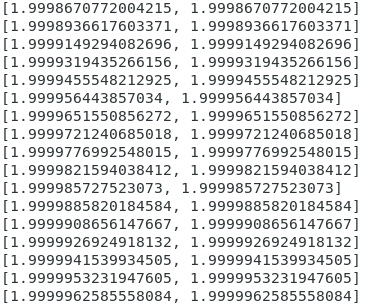
\includegraphics{HW2_samplefunc_convergence.png}
    \caption{Convergence to the minima of the sample function in equation 16. The starting values were $x=1$ and $y=1$. $\gamma$ was 10^{-2} and I used a fixed step size $h = 10^{-1}$}
    \label{fig:conv2d}
\end{figure}{}

\begin{figure}
    \centering
    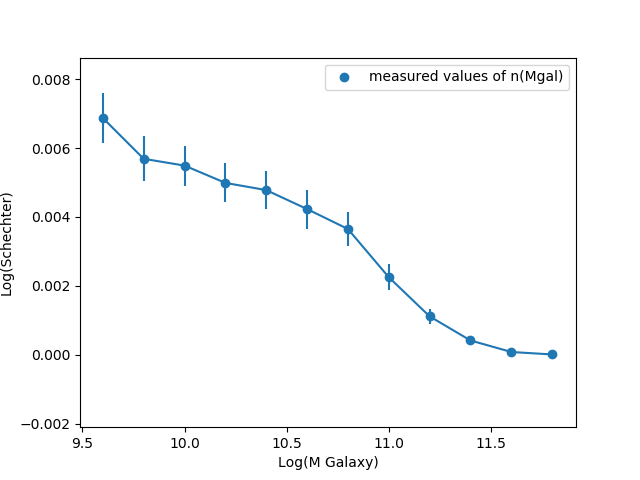
\includegraphics{HW2_schecterfit_data.png}
    \caption{Schechter function measurements $n(M_{gal})$ for different values of $M_{gal}$. Error bars are the errors of $n(M_{gal})$}
    \label{fig:data}
\end{figure}{}



\begin{figure}
    \centering
    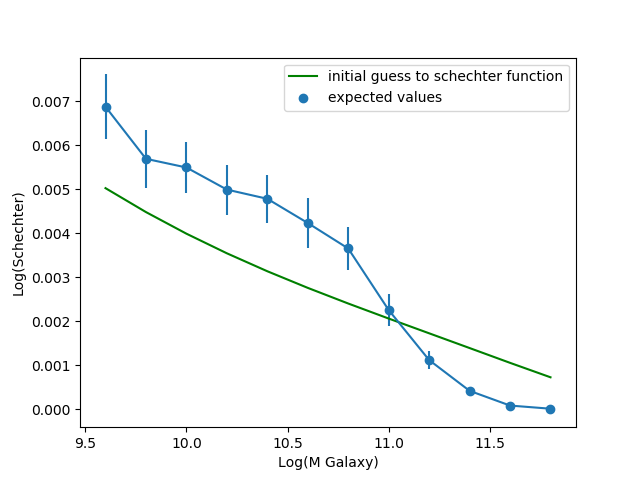
\includegraphics{HW2_schecterfit_initial.png}
    \caption{Schechter function evaluated for the initial guess parameters $\phi = 10^{-3.23}$, $M_{gal} = 10^{12}$, $\alpha = -1.243$}
    \label{fig:initial}
\end{figure}{}
\begin{figure}
    \centering
    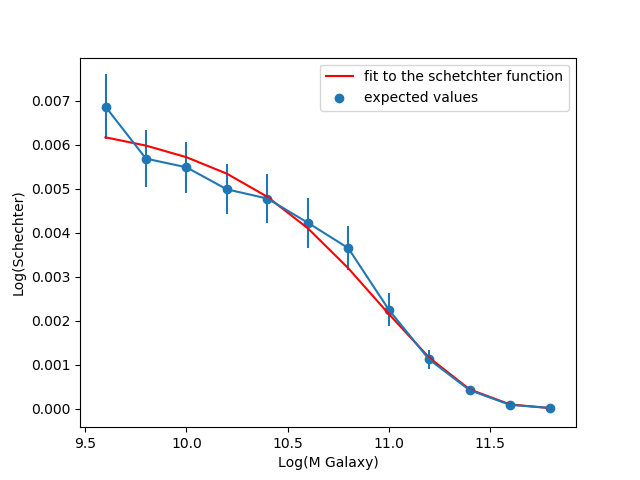
\includegraphics{HW2_schecterfit.png}
    \caption{Fit of the Schechter function with three fitting parameters. My final values were $\phi = 10^{-2.528}$, $M_{gal} = 10^{10.95}$, $\alpha = -0.943$}
    \label{fig:final}
\end{figure}{}

\begin{figure}
    \centering
    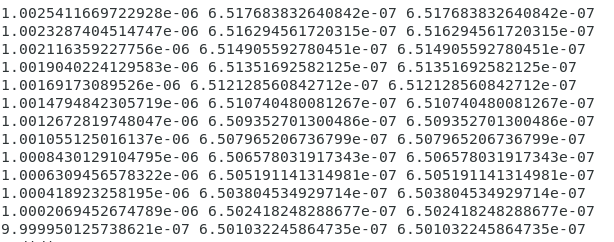
\includegraphics[width=14cm]{HW2_schecterfit_convergenceOfChi.png}
    \caption{step sizes of my gradient descent method for $\chi^2$. these show a convergance to the value $10^{-6}$ for values of the step size. We can see that a minimum $\chi^2$ is found when the step size gets lower than this tolerance.}
    \label{fig:my_label}
\end{figure}{}

\begin{figure}
    \centering
    \begin{subfigure}[b]{0.4\textwidth}
        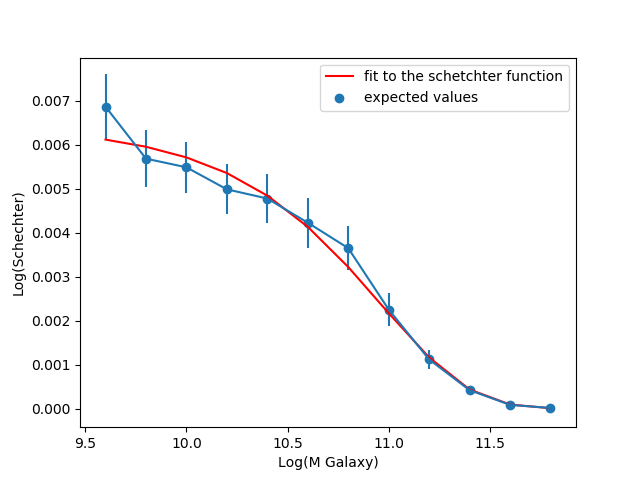
\includegraphics[width=\textwidth]{HW2_schecterfit_phi.png}
        \caption{Phi}
        \label{fig:phi}
    \end{subfigure}
    ~ 
    \begin{subfigure}[b]{0.4\textwidth}
        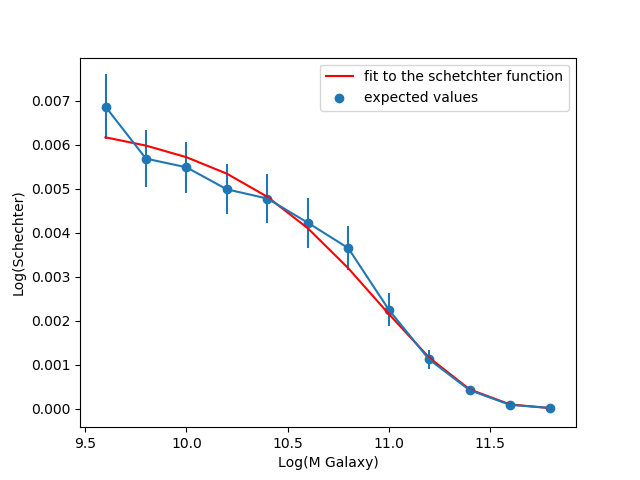
\includegraphics[width=\textwidth]{HW2_schecterfit_alpha.png}
        \caption{Alpha}
        \label{fig:alpha}
    \end{subfigure}
    ~
    \begin{subfigure}[b]{0.4\textwidth}
        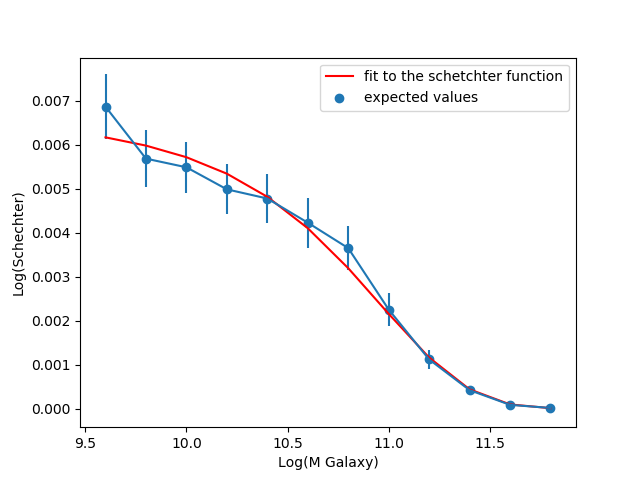
\includegraphics[width=\textwidth]{HW2_schecterfit_Mgal.png}
        \caption{Mgal}
        \label{fig:Mgal}
    \end{subfigure}
    \caption{Fits obtained by changing initial parameters, one at a time. For all the above plots I used a fixed value of $\gamma$, as well as fixed step sizes in the gradient of $chi^2$}\label{fig:animals}
\end{figure}

\begin{figure}
    \centering
    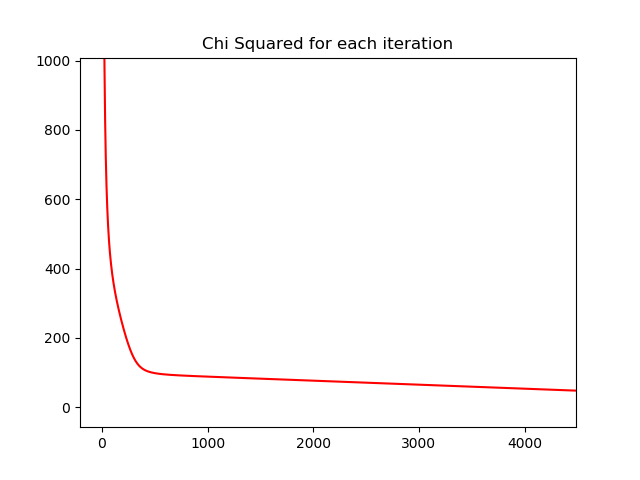
\includegraphics{HW2_schecterfit_Chiatiterations.png}
    \caption{$\chi^2$ evaluated for the initial guess parameters $\phi = 10^{-3.23}$, $M_{gal} = 10^{12}$, $\alpha = -1.243$ at every step in gradient descent process. $\gamma = 10^{-5}$ for this case, however, it should be stated that this method works for $\gamma$ up to $0.1$.\footnote{The plots are not showing up for these two values of gamma but I will include the raw plots upon submission as HW2_schecterfit_Chiatiterations_0.1.png and HW2_schecterfit_Chiatiterations_1.png respectively}}
    \label{fig:chi2}
\end{figure}{}

I will note that there is a better way of seeing the sensitivity of $\chi^2$ than the wayI did it. Since my method could only vary one paramerter at a time, keeping the other two fixed, you do not see the affect of varying two parameters at the same time. A better way to see this would be to create a contour plot of $\chi^2$ as a function of two parameters, leaving one fixed. This would tell you the minima in the function, as well as good locations to start your gradient descent method, as some initial conditions will lead the gradient descent method to diverge. 

\printbibliography




% --------------------------------------------------------------
%     You don't have to mess with anything below this line.
% --------------------------------------------------------------
 
\end{document}